%%%%%%%%%%%%%%%%%%%%%%%%%%%%% ANEXO %%%%%%%%%%%%%%%%%%%%%%%%%%%%%

%\section*{\centering{A – ANEXOS Y APÉNDICES }} % Añadir código
%\addcontentsline{toc}{section}{A - ANEXOS Y APÉNDICES}

% Los anexos y apéndices son materiales adicionales, utilizados para complementar el texto, añadidos al final del trabajo, con la finalidad de aclaración o de comprobación. Son elaborados por el autor y pretenden complementar una argumentación y sirven de fundamentación teórica, comprobación e ilustración (por ejemplo, mapas, leyes, códigos)

%\chapter*{Apendice A - }
%\label{ch:Apendice}

%\section*{\huge Apéndice A} 
%\section*{Fuentes de información para la descarga de MDT}
%\addcontentsline{toc}{chapter}{Apéndice A: Fuentes de información para descarga de MDT}

%\begin{itemize}
%	\item \item \url{https://www.cursosteledeteccion.com/fuentes-gratuitas-para-descargar-dem-modelo-de-elevacion-digital/}
%	\item \url{http://www.gisandbeers.com/descarga-de-dem-mundiales-mde/}
%	\item \url{https://gisgeography.com/free-global-dem-data-sources/}
%	\item \url{http://www.gpsvisualizer.com/elevation}
%	\item \url{https://mappinggis.com/2017/12/programas-gratuitos-para-trabajar-con-imagenes-de-satelite/}
%\end{itemize}

\newpage

\chapter{Problemas y Soluciones}

%\section*{\huge Apéndice B} 
%\section*{Problemas y Soluciones}
\label{ch:ApendiceB}
%\addcontentsline{toc}{chapter}{Apéndice B: Problemas y Soluciones}

\textit{\textbf{Nota}: La prueba se ha realizado en un macOS 10.14}\\

Como hemos venido diciendo a lo largo de los capítulos, no ha sido posible hacer uso del lenguaje estándar de consulta para información geoespacial GeoSPARQL en Protegé 5.5.0. El problema ha surgido cuando en la realización de las consultas geoespaciales no se detectaban las URIs ni lo estándares de GeoSPARQL. No obstante, previamente a haber elegido como alternativa GraphDB, se han revisado algunas vías para intentar su instalación y uso en Protegé. Por tanto, se ha estado buscando si había algún plugin con dicha librería que funcionara. \\

Lo primero que se ha encontrado ha sido ``\textit{Protegé 4 Plugin for Oracle Database}'' \footnote{The Support for Apache Jena is an adapter that provides a feature rich Java-based interface to RDF Semantic Graph that implements the well-known Apache Jena Graph, Model, BulkUpdateHandler, and DatasetGraph APIs. It supports SPARQL 1.1 and Open GeoSpatial Consortium (OGC) GeoSPARQL queries.} (\url{https://protegewiki.stanford.edu/wiki/Protege_4_Plugin_for_Oracle_Database}), plugin que supuestamente trae consigo la posibilidad de hacer consultas con GeoSPARQL, aunque sólo permite la versión 5.2 de Protegé y no la 5.5, como hemos probado de primeras. Así que nos hemos descargado la nueva versión de Protegé y el plugin de la siguiente página \footnote{\url{https://www.oracle.com/technetwork/database/options/spatialandgraph/downloads/index-156999.html}}, en donde se ha seleccionado la opción \texttt{Download Oracle Database 19c, 18c, and 12c Support for Apache Jena 3.1, Apache Jena Fuseki 2.4, and Protégé Desktop 5.2}. Al descomprimir la descarga obtenemos un directorio (\texttt{Oracle19c\_Jena-3.1.0\_Build\_20190711}) que contiene dentro una carpeta llamada \texttt{protege\_plugin}, en la cual te indica los pasos para instalar dicho plugin. Sin embargo, no ha habido éxito al seguir dichos pasos y por si acaso, se ha probado tanto para Protegé 5.5, Protegé 5.2 y Protegé 4. Por otro lado, se han buscado en Internet las maneras de instalar un plugin en Protegé, y todos indican la misma forma que viene en dicha documentación. De todas maneras se ha verificado que se haya instalado correctamente (figura \ref{fig:imagen1-comprobar}), no obstante sin éxito en su funcionamiento ya que seguía sin detectar los prefijos de GeoSPARQL (figura \ref{fig:imagen2-error}).

\begin{figure}[H]
	\centering
	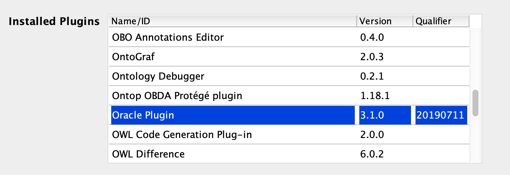
\includegraphics[width=0.8\linewidth]{imagenes/apendices/Imagen1}
	\caption{Comprobación del Plugin Oracle Database instalado}
	\label{fig:imagen1-comprobar}
\end{figure}

\begin{figure}[H]
	\centering
	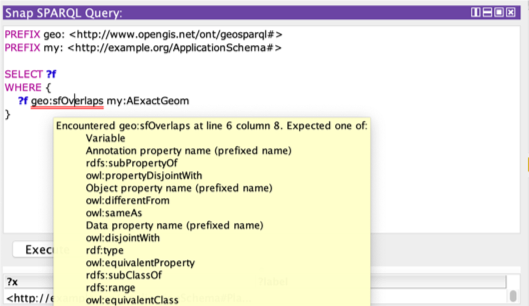
\includegraphics[width=0.85\linewidth]{imagenes/apendices/Imagen2}
	\caption{Error de GeoSPARQL en Protegé}
	\label{fig:imagen2-error}
\end{figure}

Por otra parte, para asegurar de que la consulta de GeoSPARQL en Protegé que se estaba realizando era correcta se ha usado un ejemplo proporcionado por el organismo de estándares OGC (\url{https://www.opengeospatial.org/standards/geosparql}) y al probarlo en otra herramienta se ha podido verificar que funcionaba. Pero al no conseguir éxito en Protegé, se han buscado otros softwares que permitieran hacer uso del lenguaje GeoSPARQL. De primeras se han buscado herramientas recomendadas para hacer uso de GeoSPARQL, y la que aparecía con más frecuencia era \textbf{GraphDB} (\url{https://www.ontotext.com/products/graphdb/#Try-GraphDB}). Además, es una de las que aconseja la página de Wikipedia (\url{https://en.wikipedia.org/wiki/OGC_GeoSPARQL}). Por eso mismo nos hemos descargado la versión gratuita del programa e instalado (se necesita tener Java instalado con una determinada versión y requisitos especiales), al instalarse se abre en un servidor, por lo que todo se maneja desde el navegador y se ha vuelto a probar el ejemplo de antes (\url{http://graphdb.ontotext.com/documentation/standard/geosparql-support.html#plugin-control-predicates}) y con GraphDB sí que ha funcionado (figura \ref{fig:imagen3-funciona}). En el \texttt{Apéndice \ref{ch:ApendiceC}} es posible ver la instalación de este software.

\begin{figure}[H]
	\centering
	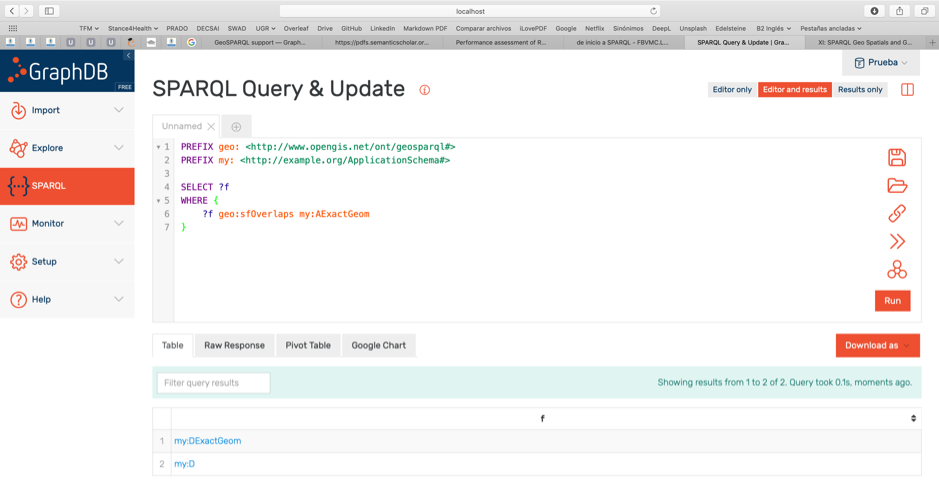
\includegraphics[width=1\linewidth]{imagenes/apendices/Imagen3}
	\caption{Comprobación del funcionamiento de GeoSPARQL en GraphDB}
	\label{fig:imagen3-funciona}
\end{figure}

Se observa como en la figura \ref{fig:imagen3-funciona}, dicho software nos permite hacer uso del lenguaje de consulta GeoSPARQL, así como una interfaz muy intuitiva y sencilla.



%Sin embargo, para hacer uso de GeoSPARQL todos hacen uso de ficheros “.rdf” y no de ficheros “.owl”, no sé si eso tiene algo que ver o si dificulta, el único problema que yo crearía la ontología con Protegé, pero no me deja sacar la salida para RDF, sino es para OWL. De todas maneras el contenido del fichero para obtener esa salida anterior es (geosparql-example.rdf). Qué según veo mete los datos distintos a como los estaba metiendo yo, ya que tendría que sacar las coordenadas de los polígonos, puntos y líneas para meterlos dentro.

%Durante la búsqueda de alternativas a Protegé para GeoSPARQL se han encontrado otras herramientas, pero debido a su dificultad se han descartado.

%Alternativas a usar GeoSPARQL sin Protegé

%ALTERNATIVA 1
%•	Por otro lado, he estado buscando otras maneras de hacer lo que quiero, y he dado con una tesis que hace algo parecido. En ese documento, lo que se hace es a partir del SHP generar los RDF, es decir, que si yo tengo un SHP para Edificaciones y otro para Curvas de Nivel, lo que consigo mediante una herramienta es obtener el RDF asociado (pero eso hace que no cree la ontología yo, problema por el que voy a seguir con la primera parte de antes comentada).
%o	Para obtener el RDF a partir de SHP hacen uso de la librería geometry2rdf (http://mayor2.dia.fi.upm.es/oeg-upm/index.php/es/technologies/151-geometry2rdf/index.html). Pero lo he estado probando y me da error, porque necesita una base de datos. Además, aquí te muestra una herramienta que hace uso de eso https://github.com/GeoKnow/TripleGeo.
%o	También hacen uso de GeoKettle, pero no sé muy bien como funciona. Es un programa que viene en OSGeoLive y que he estado probando (https://live.osgeo.org/archive/10.5/es/overview/geokettle_overview.html), y que tiene la misma funcionalidad que antes, se desea obtener el RDF.
%ALTERNATIVA 2
%•	He encontrado en Internet a través de este PDF https://event.cwi.nl/eswc2015-geo/06-publishing-handson.pdf que para pasar de SHP a RDF es posible usar GeoTriples, pero no lo he probado:
%o	https://github.com/LinkedEOData/GeoTriples
%ALTERNATIVA 3
%•	Me he metido en este enlace https://www.w3.org/wiki/ConverterToRdf, y me dice que Datalift permite pasar de SHP a RDF.


